%!TEX root = ../Thesis.tex

% 4. Analysis
% Your analysis, along with your discussion, will form the high light of your thesis. In the IMRaD format, this section is titled “Results”. This is where you report your findings and present them in a systematic manner. The expectations of the reader have been built up through the other chapters, make sure you fulfill these expectations.

% To analyse means to distinguish between different types of phenomena – similar from different. Importantly, by distinguishing between different phenomena, your theory is put to work. Precisely how your analysis should appear, however, is a methodological question. Finding out how best to organise and present your findings may take some time. A good place to look for examples and inspiration is repositories for master’s theses.

% If you are analysing human actions, you may want to engage the reader’s emotions. In this case it will be important to choose analytical categories that correlate to your chosen theory. Engaging emotions is not the main point, but a way to elucidate the phenomenon so that the reader understands it in a new and better way.

% Note: Not all theses include a separate chapter for analysis.

\chapter{Analysis}

\section{Pump control}
To check declared functionality of pump control I have made a test setup where motor's thermoresistors can replaced with matched potentiometers. In this manner I could fully control the temperatures sensed in the very beginning of the system and what is important without any modifications to the final version of the software.
\newline
\newline
I have captured 10 state transitions to demonstrate the whole spectrum of changes as follows.
\begin{description}
    \item[Temperature set to 30\textdegree C and varying accelerator displacement] \hfill \\ Expected behaviour of pumps output would be to raise proportionally from 2,5V for pedal in initial position up to 5V whenever it is pressed up to its limit.
    \item[Temperature set to 35\textdegree C and varying accelerator displacement] \hfill \\ Same behaviour as explained above.
    \item[Temperature set to 40\textdegree C and varying accelerator displacement] \hfill \\ Same behaviour as explained above.
    \item[Temperature set to 45\textdegree C and varying accelerator displacement] \hfill \\ Initial pump output should equal to $2,5V + 2,5V*25\% = 3,125V$ and saturate on pedal displacement of $75\% $.
    \item[Temperature set to 50\textdegree C and varying accelerator displacement] \hfill \\ Initial pump output should equal to $2,5V + 2,5V*50\% = 3,75V$ and saturate on pedal displacement of $50\% $.
    \item[Temperature set to 55\textdegree C and varying accelerator displacement] \hfill \\ Initial pump output should equal to $2,5V + 2,5V*75\% = 4,375V$ and saturate on pedal displacement of $25\% $.
    \item[Temperature set to 60\textdegree C and varying accelerator displacement] \hfill \\ Initial pump output should equal to maximum value of $5V$ and pedal displacement should not affect this value.
    \item[Temperature set to 65\textdegree C and varying accelerator displacement] \hfill \\ Same behaviour as explained above.
    \item[Temperature set to 70\textdegree C and varying accelerator displacement] \hfill \\ Same behaviour as explained above.
\end{description}
\begin{description}
    \item[Varying temperature from 30 to 70 degrees and no accelerator displacement] \hfill \\ Pump output should vary from $2,5V$ and $5V$ being in direct proportion to temperature changes from 40 to 60 degrees.
\end{description}

Taking for instance measurement for temperature set $50\deg C$ and pressing acceleration pedal. I have had captured extremely noisy signal from accelerator sensor and temperature sensor emulator then prepossessed in similar manner as it is done inside the system (just to filter out the electromagnetic noise \todo{Precise description?}). The sensors output as well as pumps controlling signal has been shown in the figure \ref{pump_50}.

\begin{figure}[h]
    \centering
    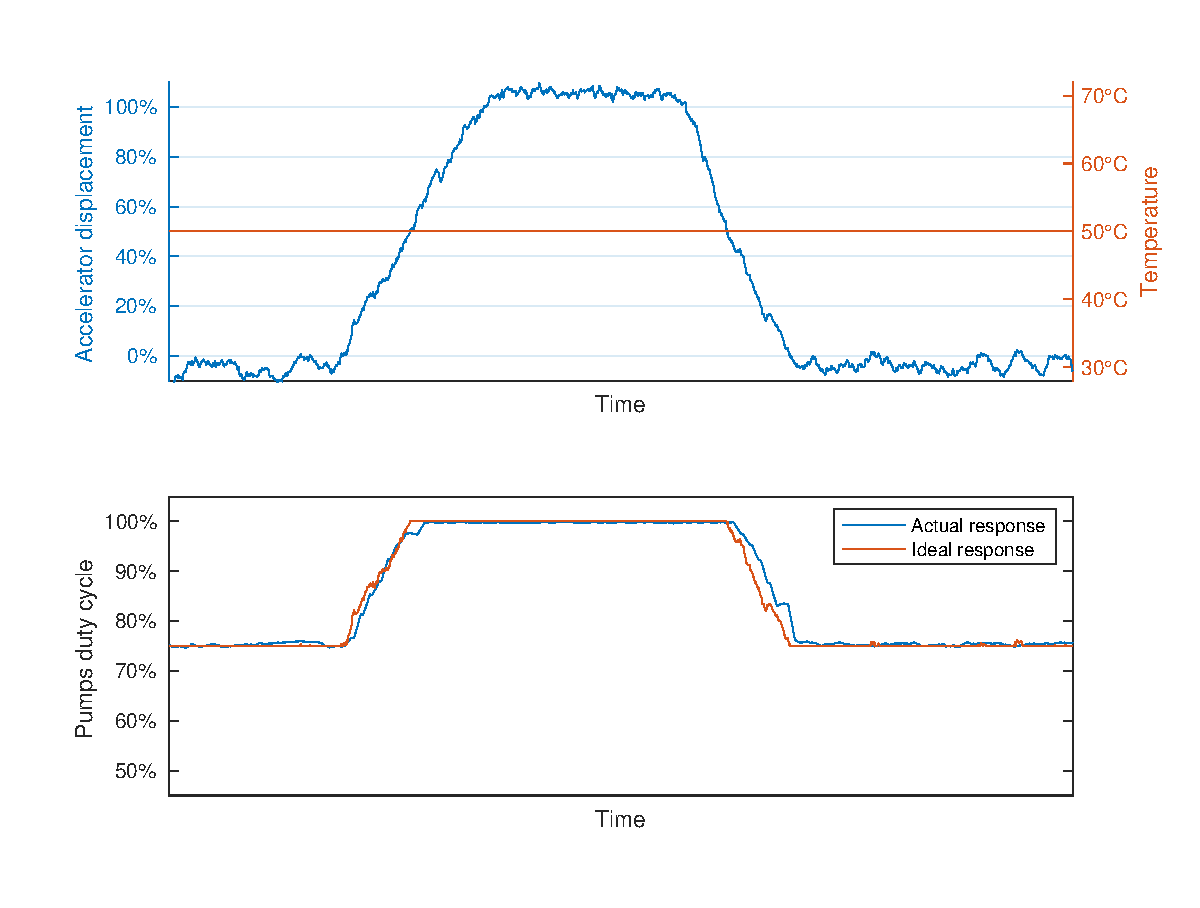
\includegraphics[height=5.8cm]{figures/pump_50.eps}
    \caption[Temperature set to 50\textdegree C and varying accelerator displacement]{Comparison of actual pump control signal to idealised one based on the same input data}
    \label{pump_50}
\end{figure}

In the same figure I have plot theoretical output based on idealised mathematical model. As one can notice control output closely follows desired patch. The only visible difference is due to the fact that in my system the control signal is intentionally delayed.
The pumps control signal is updated only once per 100 millisecond since temperature change is rather slow process in this way we can avoid harmful (for pumps) high frequency oscillations and save computation power. In this way we obtain simple control system with memory which is even more visible if we just plot input against output (accelerator/control signal) which has been done in \ref{pump_50_1}. In the graph we can observe the hysteresis and steps upon control update as we could expect.


\begin{figure}[h]
    \centering
    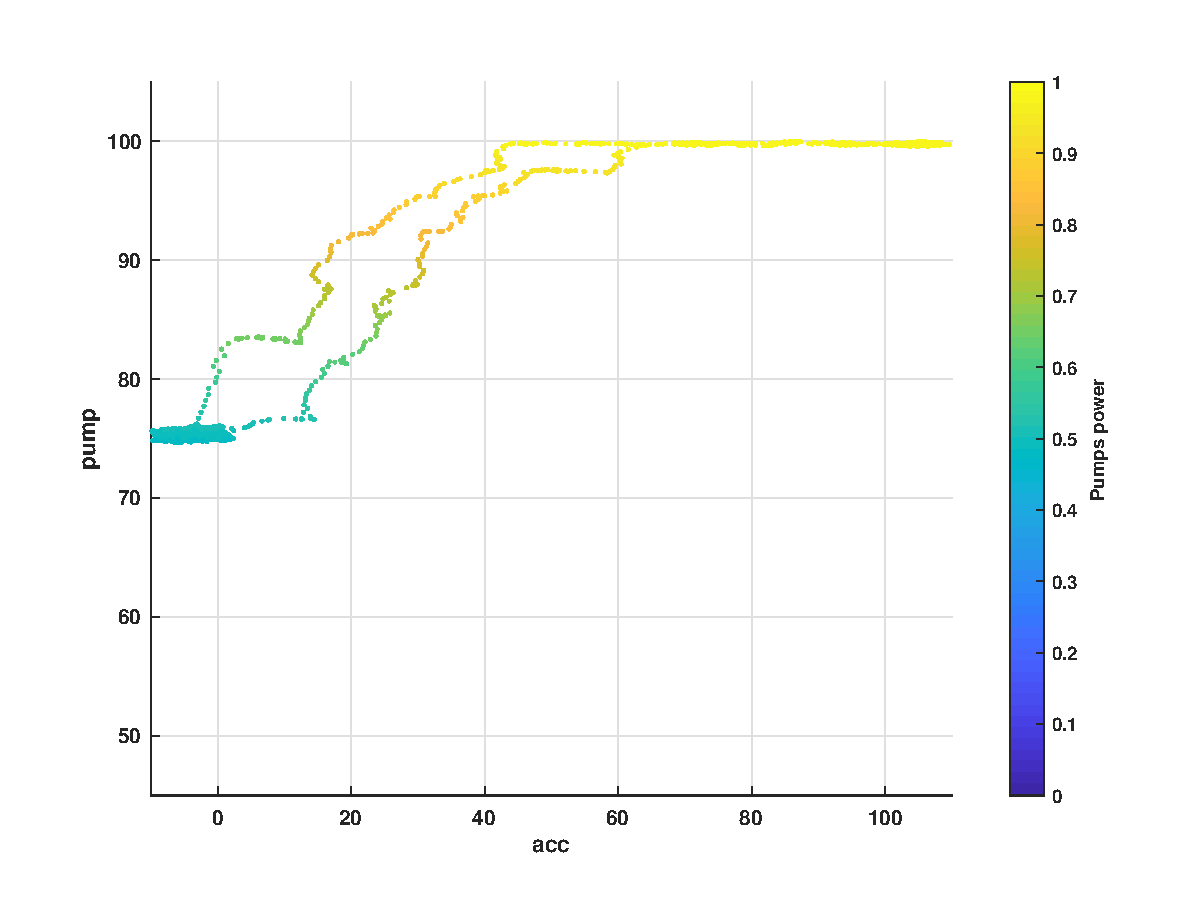
\includegraphics[height=5.8cm]{figures/pump_50_1.eps}
    \caption[Accelerator displacement against pump output]{Accelerator displacement against pump output (samples sorted based accelerator position)}
    \label{pump_50_1}
\end{figure}

I have repeat this process for all above mentioned cases confirming that this sub-system works correctly. The figures for all the other cases can be found in appendix \todo{Appendix pumps}. To present all the results in clear graphical way I have combined them into scatter chart plotting the accelerator against temperature values and colour mapping them by measured output \ref{Raw_pump_sum}. To show the validity of data on the right you can see the same graph with the background coloured based on mathematical model.

\begin{figure}[h]
    \centering
        \subbottom[Measured controlling signal]{
            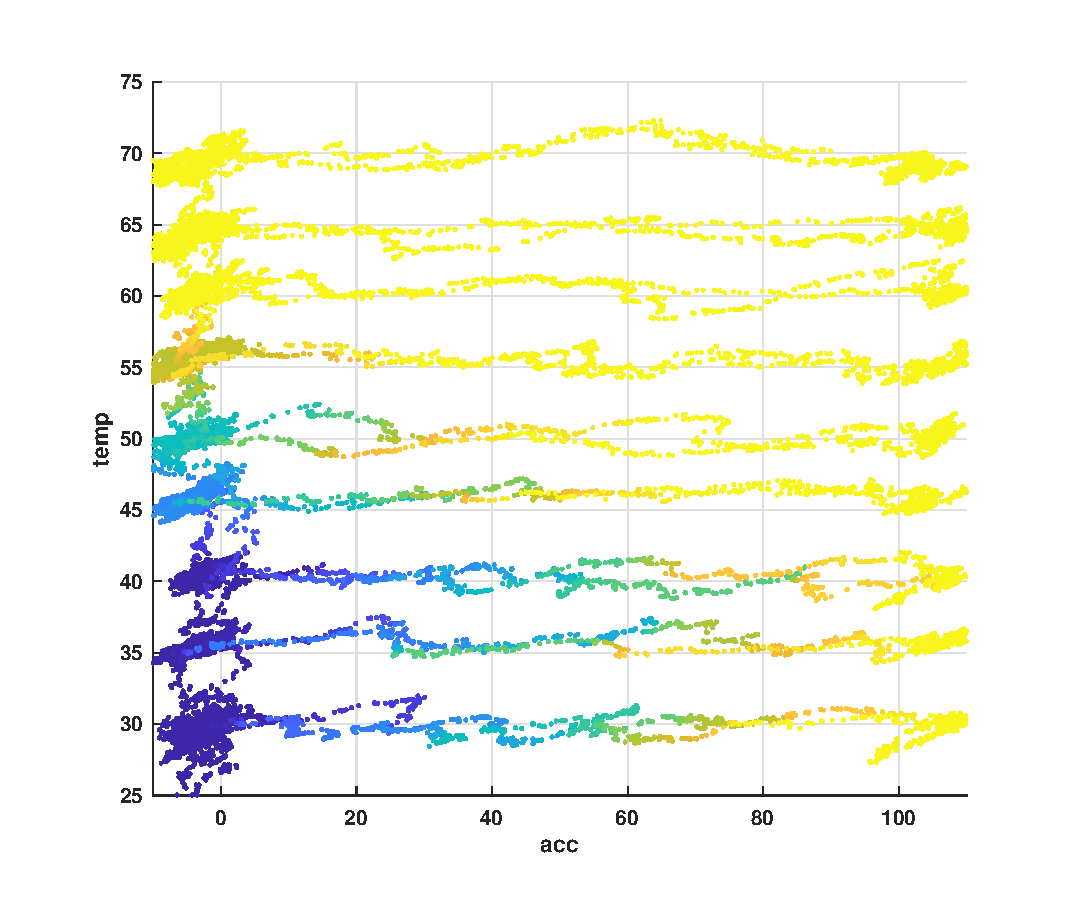
\includegraphics[height=5.8cm]{figures/Pumps_summary_raw.eps}
            \label{Raw_pump_sum}
        }
        ~
        \subbottom[With shading based on the model]{
            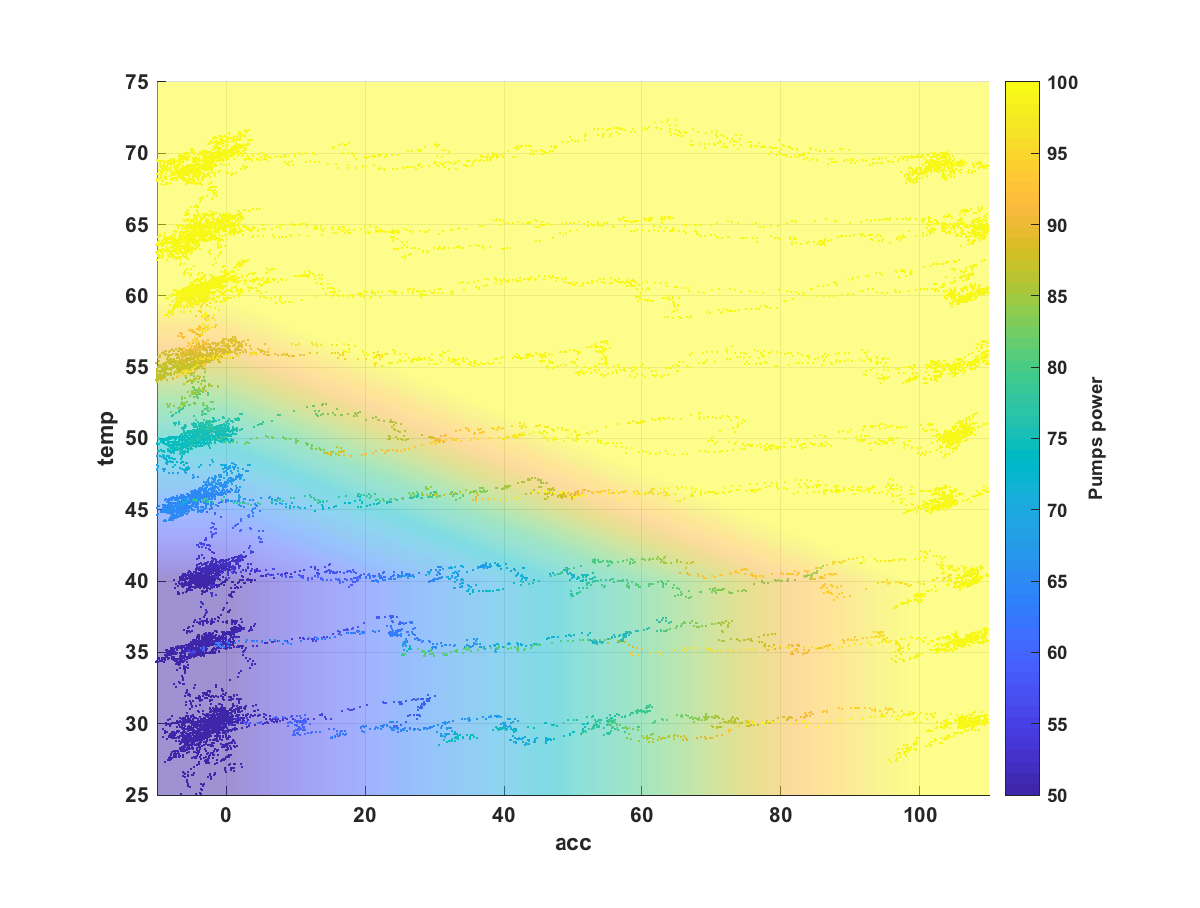
\includegraphics[height=5.8cm]{figures/Pumps_summary.eps}
            \label{Shaded_pump_sum}
        }
        \caption{Pumps control summary}
    \label{Pump_sum}
\end{figure}









Measured interval at which the pedals and steering wheel status is send is equal to $6,8ms$.